\chapter{Bell inequalities and nonlocality}\label{ch:bell}

\section{The EPR argument}
In 1935 Einstein, Podolsky and Rosen (EPR) \cite{EPR1935} argued that quantum mechanics might be an incomplete description of reality. In the form
given by Bohm, the argument goes as follows. Two spin-$\frac12$ particles are prepared in the singlet state and fly apart. If Alice measures $\sigma_z$ on
her particle, she can predict with certainty the result of a measurement of $\sigma_z$ on Bob's particle (the opposite one), without disturbing it in any way,
if the two measurements are space-like separated. According to EPR, the value of $\sigma_z$ of Bob's particle is then an ``element of reality''. But Alice
could equally well have measured $\sigma_x$, so $\sigma_x$ of Bob's particle must also be an element of reality. Quantum mechanics does not allow both
values to be defined simultaneously ($[\sigma_x,\sigma_z]\neq0$), so, EPR concluded, it must be incomplete: it should be completed by additional
\emph{hidden variables}.

In 1964 John Bell \cite{Bell1964} took the EPR thought experiment one step further. He showed that the question is not merely philosophical: if the hidden
variables are \emph{local}, they lead to predictions that can be tested experimentally, and that contradict quantum mechanics.

\section{The setup and the quantum prediction}
A source emits pairs of spin-$\frac12$ particles in the singlet state
\begin{equation}
  \ket{\psi^-}=\frac1{\sqrt2}\left(\ket{\uparrow\downarrow}-\ket{\downarrow\uparrow}\right),
\end{equation}
which fly apart in opposite directions (\cref{fig:bellsetup}). One particle reaches Alice's analyzer, which measures the spin component along a unit
vector $\vec a$; the other reaches Bob's analyzer, oriented along $\vec b$. Each measurement gives the result $+1$ or $-1$ (in units of $\hbar/2$).

\begin{figure}[h]\centering
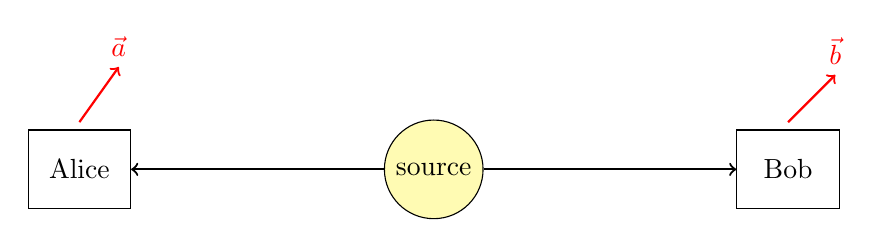
\begin{tikzpicture}
  \node[draw,circle,fill=yellow!30] (s) at (0,0) {source};
  \node[draw,rectangle,minimum width=1.3cm,minimum height=1cm] (a) at (-4.5,0) {Alice};
  \node[draw,rectangle,minimum width=1.3cm,minimum height=1cm] (b) at (4.5,0) {Bob};
  \draw[->,thick] (s)--(a); \draw[->,thick] (s)--(b);
  \draw[->,red,thick] (-4.5,0.6)--(-4.0,1.3) node[above]{$\vec a$};
  \draw[->,red,thick] (4.5,0.6)--(5.1,1.2) node[above]{$\vec b$};
\end{tikzpicture}
\caption{A Bell experiment. A pair of particles emitted by the source is analyzed along the directions $\vec a$ and $\vec b$, which can be chosen freely.}
\label{fig:bellsetup}
\end{figure}

Bell's simple but powerful idea was to consider the average of the product of the two results, the \emph{correlation function} $P(\vec a,\vec b)$.
\begin{proposition}
For the singlet state,
\begin{equation}\label{eq:singletcorr}
  P_{\rm QM}(\vec a,\vec b)=\mel{\psi^-}{(\vec a\cdot\vec\sigma)\otimes(\vec b\cdot\vec\sigma)}{\psi^-}=-\vec a\cdot\vec b.
\end{equation}
\end{proposition}
\begin{proof}
The singlet has total spin zero: $(\vec\sigma\otimes I+I\otimes\vec\sigma)\ket{\psi^-}=0$, which can be checked component by component (e.g.\
$(Z\otimes I+I\otimes Z)(\ket{01}-\ket{10})=(1-1)\ket{01}-(-1+1)\ket{10}=0$). Therefore $(I\otimes\vec b\cdot\vec\sigma)\ket{\psi^-}=-(\vec b\cdot\vec\sigma\otimes I)\ket{\psi^-}$ and
\begin{equation}
  P_{\rm QM}=-\mel{\psi^-}{(\vec a\cdot\vec\sigma)(\vec b\cdot\vec\sigma)\otimes I}{\psi^-}
  =-\vec a\cdot\vec b-\ii(\vec a\times\vec b)\cdot\mel{\psi^-}{\vec\sigma\otimes I}{\psi^-}=-\vec a\cdot\vec b,
\end{equation}
where we used the product rule of Pauli matrices and the fact that each particle alone is completely unpolarized,
$\mel{\psi^-}{\vec\sigma\otimes I}{\psi^-}=0$ (its reduced density matrix is $I/2$, \cref{ch:density}).
\end{proof}
If the angle between the analyzers is $\theta_{ab}$, $P=-\cos\theta_{ab}$, and the probability of equal results is $P(A=B)=\frac{1+P}2=\sin^2\frac{\theta_{ab}}2$.
The antiparallel and parallel configurations recover the EPR situation:
\begin{equation}
  P(\vec a,-\vec a)=+1,\qquad P(\vec a,\vec a)=-1.
\end{equation}
If both analyzers are along the same axis, the results are always opposite, so measuring one particle allows us to predict with certainty the result for the other.
Note, however, that each result alone is completely random: $P(A=+1)=1/2$ for any $\vec a$.

\section{Local hidden variables and Bell's inequality}
Assume now that the wave function is not the complete description, and that each pair also carries some unknown variables, collectively denoted $\lambda$,
distributed with a probability density $\rho(\lambda)\ge0$, $\int\rho(\lambda)\dd\lambda=1$. In such a complete theory the results of the measurements
are determined by $\lambda$:
\begin{equation}
  A(\vec a,\lambda)=\pm1,\qquad B(\vec b,\lambda)=\pm1.
\end{equation}
The essential assumption is \emph{locality}: Alice's result $A$ depends only on her own setting $\vec a$ and on $\lambda$, but not on Bob's setting $\vec b$,
and vice versa. A second, implicit, assumption is \emph{measurement independence} (``free will''): $\rho(\lambda)$ does not depend on the settings. The correlation
function is then
\begin{equation}\label{eq:lhvcorr}
  P(\vec a,\vec b)=\int\rho(\lambda)A(\vec a,\lambda)B(\vec b,\lambda)\dd\lambda.
\end{equation}
To reproduce the perfect EPR anticorrelations, the hidden variables must satisfy $A(\vec a,\lambda)=-B(\vec a,\lambda)$ for all $\vec a,\lambda$.

\paragraph{Derivation.} Substituting $B=-A$,
\begin{equation}
  P(\vec a,\vec b)=-\int\rho(\lambda)A(\vec a,\lambda)A(\vec b,\lambda)\dd\lambda .
\end{equation}
Introducing a third orientation $\vec c$,
\begin{equation}
  P(\vec a,\vec b)-P(\vec a,\vec c)=-\int\rho(\lambda)\left[A(\vec a,\lambda)A(\vec b,\lambda)-A(\vec a,\lambda)A(\vec c,\lambda)\right]\dd\lambda.
\end{equation}
Since $A(\vec b,\lambda)^2=1$, we can factor out $A(\vec a,\lambda)A(\vec b,\lambda)$:
\begin{equation}
  P(\vec a,\vec b)-P(\vec a,\vec c)=-\int\rho(\lambda)\left[1-A(\vec b,\lambda)A(\vec c,\lambda)\right]A(\vec a,\lambda)A(\vec b,\lambda)\dd\lambda .
\end{equation}
Now $-1\le A(\vec a,\lambda)A(\vec b,\lambda)\le1$ and $\rho(\lambda)[1-A(\vec b,\lambda)A(\vec c,\lambda)]\ge0$. It follows that
\begin{equation}
  \abs{P(\vec a,\vec b)-P(\vec a,\vec c)}\le\int\rho(\lambda)\left[1-A(\vec b,\lambda)A(\vec c,\lambda)\right]\dd\lambda.
\end{equation}
The first term of the integral is $1$ by normalization, and the second is $P(\vec b,\vec c)$ (using $A(\vec c)=-B(\vec c)$ again). We obtain \emph{Bell's inequality}
\begin{equation}\label{eq:bellineq}
  \abs{P(\vec a,\vec b)-P(\vec a,\vec c)}\le1+P(\vec b,\vec c).
\end{equation}

\paragraph{Violation by quantum mechanics.} Take $\vec a\perp\vec b$ in a plane, with $\vec c$ at $45^\circ$ from both. Then
$P_{\rm QM}(\vec a,\vec b)=0$ and $P_{\rm QM}(\vec a,\vec c)=P_{\rm QM}(\vec b,\vec c)=-\cos45^\circ\approx-0.707$, and \cref{eq:bellineq} would require
$0.707\le1-0.707=0.293$, which is false. \emph{No local hidden-variable theory can reproduce all the predictions of quantum mechanics.}

\section{The CHSH inequality}
Bell's original inequality relies on perfect anticorrelations, which are never observed exactly in experiments. Clauser, Horne, Shimony and Holt \cite{CHSH1969}
derived an inequality without this assumption. Each side chooses between two settings, $\vec a,\vec a'$ for Alice and $\vec b,\vec b'$ for Bob. Define
\begin{equation}
  S=E(\vec a,\vec b)+E(\vec a,\vec b')+E(\vec a',\vec b)-E(\vec a',\vec b'),
\end{equation}
where $E$ is the measured correlation.
\begin{theorem}[CHSH]
In a local hidden-variable theory, $|S|\le2$.
\end{theorem}
\begin{proof}
For each $\lambda$, write $A=A(\vec a,\lambda)$, $A'=A(\vec a',\lambda)$, $B=B(\vec b,\lambda)$, $B'=B(\vec b',\lambda)$, all equal to $\pm1$. Then
\begin{equation}
  AB+AB'+A'B-A'B'=A(B+B')+A'(B-B').
\end{equation}
Either $B=B'$, and then the first bracket is $\pm2$ and the second is $0$, or $B=-B'$, and the converse. In both cases the expression is $\pm2$.
Averaging over $\lambda$ with the positive weight $\rho(\lambda)$ gives $|S|\le2$.
\end{proof}
In quantum mechanics, with the singlet, $E=-\cos\theta$. Choosing the four directions in a plane at the angles $a=0$, $a'=90^\circ$, $b=45^\circ$, $b'=-45^\circ$,
\begin{equation}
  S=-\left[\cos45^\circ+\cos45^\circ+\cos45^\circ-\cos135^\circ\right]=-2\sqrt2,\qquad|S|=2\sqrt2\approx2.83>2.
\end{equation}

\begin{theorem}[Tsirelson bound]
In quantum mechanics, $|S|\le2\sqrt2$ for any state and any measurements.
\end{theorem}
\begin{proof}
Let $A,A',B,B'$ be Hermitian with eigenvalues $\pm1$ (so $A^2=\dots=I$), acting on Alice's and Bob's spaces. The CHSH operator
$\mathcal C=A\otimes(B+B')+A'\otimes(B-B')$ satisfies (expand, using $(B\pm B')^2=2I\pm\{B,B'\}$)
\begin{equation}
  \mathcal C^2=4\,I\otimes I-[A,A']\otimes[B,B'].
\end{equation}
Since $\norm{[A,A']}\le2\norm A\norm{A'}=2$ and similarly for $B$, $\norm{\mathcal C^2}\le8$, hence $|\expval{\mathcal C}|\le\norm{\mathcal C}\le2\sqrt2$.
\end{proof}
The bound $2\sqrt2$ is reached only if $[A,A']$ and $[B,B']$ are ``maximal'', i.e.\ for anticommuting observables like $\sigma_x$ and $\sigma_z$: incompatibility of
measurements is the resource behind nonlocality. Theories with $|S|$ up to $4$ (``PR boxes'') would still forbid signalling; why nature stops at $2\sqrt2$ is an open
foundational question.

\paragraph{Photons.} For polarization-entangled photons in $\ket{\Phi^+}=(\ket{HH}+\ket{VV})/\sqrt2$ and polarizers at angles $\alpha$ and $\beta$ in real space,
$E(\alpha,\beta)=\cos2(\alpha-\beta)$ (the factor 2 is the Poincaré-sphere double angle). The maximal violation is obtained at $\alpha=0$, $\alpha'=45^\circ$,
$\beta=22.5^\circ$, $\beta'=-22.5^\circ$.

\section{Experiments and loopholes}
The question can be settled by experiment. The first tests were done by Freedman and Clauser (1972). The experiments of Aspect, Grangier and Roger \cite{Aspect1982} with
entangled photons from an atomic cascade gave $S=2.697\pm0.015$, in agreement with quantum mechanics, and a later experiment by Aspect, Dalibard and Roger switched the
settings during the flight of the photons. Real experiments must close \emph{loopholes}:
\begin{itemize}
  \item the \emph{locality loophole}: the choice of setting on one side must be space-like separated from the measurement on the other side (closed by Weihs et al.\ in 1998
  with random settings and 400\,m separation);
  \item the \emph{detection loophole}: if many particles are lost, the detected subset may be unrepresentative (closed with ions in 2001, with superconducting detectors for photons later);
  \item the \emph{freedom-of-choice loophole}: the settings must be independent of $\lambda$ (``cosmic Bell tests'' used light from distant quasars to choose them).
\end{itemize}
In 2015, three groups (Delft, with electron spins separated by 1.3\,km; Vienna and NIST, with photons) performed the first loophole-free Bell tests. The 2022 Nobel prize
in physics was awarded to A.~Aspect, J.~Clauser and A.~Zeilinger for these experiments. The conclusion is that nature is not described by any local hidden-variable theory.
This is also the foundation of device-independent random number generation and cryptography: a violation of a Bell inequality certifies that the outcomes did not exist before
the measurement, whatever the inner workings of the devices.

\paragraph{No signalling.} Nonlocal correlations do not allow faster-than-light communication. Bob's marginal probabilities do not depend on Alice's choice of setting:
$\sum_AP(A,B|\vec a,\vec b)=P(B|\vec b)$, because Bob's reduced density matrix is not changed by operations on Alice's side (\cref{ch:density}). The correlations appear only
when the two lists of results are compared, which requires a classical channel.

\section{GHZ: nonlocality without inequalities\starred}
For three qubits in $\ket{\rm GHZ}=(\ket{000}+\ket{111})/\sqrt2$ one checks, using $X\ket0=\ket1$, $Y\ket0=\ii\ket1$, $Y\ket1=-\ii\ket0$,
\begin{equation}
  XXX\ket{\rm GHZ}=+\ket{\rm GHZ},\qquad XYY\ket{\rm GHZ}=YXY\ket{\rm GHZ}=YYX\ket{\rm GHZ}=-\ket{\rm GHZ}.
\end{equation}
A local hidden-variable model would assign values $x_i,y_i=\pm1$ to each qubit. The last three relations require $x_1y_2y_3=y_1x_2y_3=y_1y_2x_3=-1$; their product is
$x_1x_2x_3(y_1y_2y_3)^2=x_1x_2x_3=-1$, in contradiction with the first relation, which requires $+1$. A single run of the experiment contradicts local realism
(Greenberger, Horne, Zeilinger 1989; Mermin 1990).

\section{Entanglement-based QKD: Ekert's protocol (E91)}\label{sec:e91}
Ekert \cite{Ekert1991} proposed in 1991 a key distribution protocol in which the security is tested by a Bell inequality.
\begin{enumerate}
  \item A source (which may even be controlled by Eve) distributes pairs of qubits, ideally in the singlet state, one to Alice and one to Bob.
  \item Alice measures her qubit along one of three directions in the $xz$ plane of the Bloch sphere, chosen at random, at angles $a_1=0$, $a_2=45^\circ$, $a_3=90^\circ$.
  Bob measures along $b_1=45^\circ$, $b_2=90^\circ$, $b_3=135^\circ$. (For polarization photons, divide the angles by two.)
  \item They announce their choices of directions publicly. In the cases where they used the same direction ($a_2=b_1$ or $a_3=b_2$, a fraction $2/9$ of the pairs)
  their results are perfectly anticorrelated, and Bob flips his bit: this is the \emph{key}.
  \item With the results for $(a_1,a_3)\times(b_1,b_3)$, they compute the CHSH quantity
  \begin{equation}
    S=E(a_1,b_1)-E(a_1,b_3)+E(a_3,b_1)+E(a_3,b_3),
  \end{equation}
  which for the singlet equals $-2\sqrt2$ (check it with $E=-\cos(a-b)$). The remaining combinations are discarded.
\end{enumerate}
\paragraph{Why it is secure.} If Eve gains information about the outcomes, for instance by measuring the particles in transit, or by preparing the pairs in states with
predetermined values, the correlations become those of a local hidden-variable model with $\lambda$ = Eve's information, and then $|S|\le2$. Observing $|S|=2\sqrt2$
therefore guarantees that the outcomes did not exist before the measurements and are unknown to anybody. More quantitatively, the monogamy of entanglement implies that
if Alice and Bob are maximally entangled, Eve is uncorrelated with them. The key is created at the moment of measurement and is never ``sent'': it does not exist
before. This is the first device-independent idea in quantum cryptography. For identical devices and the singlet source, E91 is equivalent to BB84 (Bennett, Brassard,
Mermin 1992): Alice's measurement prepares Bob's qubit in one of the BB84 states.

\section{Exercises}
\begin{exercise}
Show that for $\ket{\Phi^+}$, $\mel{\Phi^+}{(\vec a\cdot\vec\sigma)\otimes(\vec b\cdot\vec\sigma)}{\Phi^+}=a_xb_x-a_yb_y+a_zb_z$. Find settings that give $|S|=2\sqrt2$.
\end{exercise}
\begin{exercise}
For the \emph{Werner state} $\rho=p\proj{\psi^-}+(1-p)I/4$, show that the maximal CHSH value is $2\sqrt2\,p$. Hence the state violates CHSH only if $p>1/\sqrt2$,
although it is entangled for $p>1/3$ (\cref{ex:werner}).
\end{exercise}
\begin{exercise}
Construct an explicit local hidden-variable model that reproduces the perfect anticorrelations $P(\vec a,\vec a)=-1$ and gives $P(\vec a,\vec b)=-1+2\theta_{ab}/\pi$
(the ``linear'' correlation). Compare with $-\cos\theta_{ab}$. (Hint: $\lambda$ is a random unit vector, and $A=\operatorname{sign}(\vec a\cdot\vec\lambda)$, $B=-\operatorname{sign}(\vec b\cdot\vec\lambda)$.)
\end{exercise}
